\documentclass[10pt]{beamer}
\usepackage{amsmath,amssymb,longtable,hhline}
\usepackage{mathrsfs}
\usepackage{hyperref}
\usepackage{xcolor}
\usepackage{multicol}
\usepackage{anyfontsize}
\usepackage{minted}

\usemintedstyle{tango}
\RequirePackage{polyglossia}
\RequirePackage{indentfirst}
\RequirePackage[protrusion=false,expansion=false]{microtype}
\SetProtrusion
    [name=std]
    {
      encoding={utf8},
      family=*}
    {
    « = {300,     },
    » = {    , 300},
    „ = {300,     },
    “ = {    , 300},
    ( = {300,     },
    ) = {    , 300},
    ! = {    , 300},
    ? = {    , 300},
    : = {    , 300},
    ; = {    , 300},
    . = {    , 300},
    - = {    , 300},
й   {,}= {    , 300}
    }
%\DeclareMicrotypeSet{t2atext}{}
%\UseMicrotypeSet{t2atext}
\microtypesetup{protrusion=true,expansion=true}
\newfontfeature{Microtype}{protrusion=default;expansion=default;}

\setmainlanguage{russian}
\setotherlanguage{english}
\setkeys{russian}{babelshorthands=true}
\usepackage{minted}


\newcommand{\ltprgsize}{\fontsize{5}{5}\selectfont}
%\newcommand{\ltprgsize}{\footnotesize}
\setminted{fontsize=\footnotesize{},mathescape}

\definecolor{mygreen}{rgb}{0,0.6,0}
\definecolor{mygray}{rgb}{0.5,0.5,0.5}
\definecolor{mymauve}{rgb}{0.58,0,0.82}

\hypersetup{
    bookmarks=true,         % show bookmarks bar?
    unicode=true,           % non-Latin characters in Acrobat’s bookmarks
    pdftoolbar=false,        % show Acrobat’s toolbar?
    pdfmenubar=false,        % show Acrobat’s menu?
    pdffitwindow=false,     % window fit to page when opened
    pdfstartview={FitH},    % fits the width of the page to the window
    pdftitle={Model Driven Architecture Implementation using Linked Data},    % title
    pdfauthor={Evgeny Cherkashin, Alexey Kopaygorodsky, Ljubica Kazi, Alexey Shigarov, Viacheslav Paramonov},     % author
    pdfsubject={model driven architecture},   % subject of the document
    pdfnewwindow=true,      % links in new PDF window
    colorlinks=true,       % false: boxed links; true: colored links
    linkcolor=red,          % color of internal links (change box color with linkbordercolor)
    citecolor=green,        % color of links to bibliography
    filecolor=magenta,      % color of file links
    urlcolor=blue           % color of external links
}

\usepackage{pifont}

\usetheme{Warsaw}
\usecolortheme{crane}
%\useinnertheme{rectangles}
%\setbeamertemplate{itemize item}{\scriptsize\hbox{\donotcoloroutermaths\ding{113}}}
\definecolor{darkding}{RGB}{200,56,0}
\setbeamertemplate{itemize item}{\scriptsize\hbox{\color{darkding}{\bfseries\ding{113}}}}
\setbeamertemplate{itemize subitem}{\tiny\raise1.5pt\hbox{\donotcoloroutermaths$\blacktriangleright$}}
\setbeamertemplate{itemize subsubitem}{\tiny\raise1.5pt\hbox{\donotcoloroutermaths$\blacktriangleright$}}
\setbeamertemplate{enumerate item}{\insertenumlabel.}
\setbeamertemplate{enumerate subitem}{\insertenumlabel.\insertsubenumlabel}
\setbeamertemplate{enumerate subsubitem}{\insertenumlabel.\insertsubenumlabel.\insertsubsubenumlabel}
\setbeamertemplate{enumerate mini template}{\insertenumlabel}

\beamertemplatenavigationsymbolsempty

\usepackage{iftex,ifxetex}
\ifPDFTeX
  \usepackage[utf8]{inputenc}
  \usepackage[T1]{fontenc}
  \usepackage[russian]{babel}
  \usepackage{lmodern}
  \usefonttheme{serif}
\else
  \ifluatex
    \usepackage{unicode-math}
    \defaultfontfeatures{Ligatures=TeX,Numbers=OldStyle}
    \setmathfont{Latin Modern Math}
    \setsansfont{Linux Biolinum O}
    \setmonofont{Fira Mono}[Scale=MatchLowercase]
    \usefonttheme{professionalfonts}
    % \setmathfont[
    %     Ligatures=TeX,
    %     Scale=MatchLowercase,
    %     math-style=upright,
    %     vargreek-shape=unicode
    %     ]{euler.otf}
    % \newfontfamily{\cyrillicfont}{Times New Roman}
    % \newfontfamily{\cyrillicfontrm}{Times New Roman}
    % \newfontfamily{\cyrillicfonttt}{Courier New}
    % \newfontfamily{\cyrillicfontsf}{Arial}
    \newfontfamily{\cyrillicfont}{Linux Biolinum O}
    \newfontfamily{\cyrillicfontrm}{Linux Biolinum O}
    \newfontfamily{\cyrillicfonttt}{Fira Mono}
    \newfontfamily{\cyrillicfontsf}{Fira Sans}
  \fi
\fi

%\useoutertheme{split}
%\useinnertheme{rounded}
\setbeamertemplate{background canvas}[vertical shading][bottom=white!80!cyan!20,top=cyan!10]
%\setbeamertemplate{sidebar canvas left}[horizontal shading][left=white!40!black,right=black]

\graphicspath{{pics/}}

\providecommand{\email}[1]{\text{#1}}

% --------------------------




\begin{document}

\setbeamertemplate{background canvas}[vertical shading][bottom=white,top=white]
\setbeamercolor{background canvas}{bg=white}

\title[Инструментарий для анализа текстовых сцен]{Инструментарий анализа, классификации и интерпретации
сцен}
\author{\bfseries%
Евгений Черкашин \\ \email{\href{mailto:eugeneai@icc.ru}{eugeneai@icc.ru}}}
\institute{\normalsize г.~Иркутск, Институт динамики систем и теории управления им. В.~М.~Матросова СО РАН\\[1em]%
}
\date[2022c]{{}\\\footnotesize
Применение методов классификации с использованием технологий искусственного интеллекта для семантической интерпретации текстовых данных в системах автоматизации деятельности органов военного управления}
%\date{\today}
\maketitle
\begin{frame}
  \frametitle{Современное состояние}
  \begin{itemize}
  \item В настоящий момент ИИ чаще всего -- это машинное обучение: нейронные сети
    \begin{itemize}
    \item алгоритмические структуры свертки
    \item генерирующие нейронные сети
    \item модели регрессии, таксономии, классификации на основе машинного обучения и т.~п.
    \end{itemize}
  \item известное ограничение -- невозможность интерпретации получаемых моделей в виде процедуры трансформации данных. ИНС -- это набор коэффициентов.
  \item другое ограничение -- сложность построения моделей для меняющихся во времени объектов (\emph{динамических объектов и систем}).
Например, последовательность сообщений между участниками общения может формировать некоторый план саботажа промышленного объекта.
  \end{itemize}

  Построение моделей АКИД на основе логического программирования (СОЗ) позволяет продвинуться в решении задач распознавания на основе сценариев.
\end{frame}
\begin{frame}
  \frametitle{Цели исследования}
  \textbf{Основная цель} НИРОКР -- разработка технологии анализа текстов, базирующихся на формализованных знаниях. Решаются следующие основные проблемы:
  \begin{enumerate}
  \item разработка методик анализа, классификации и интерпретации данных (АКИД), полученных на этапах применения машинного обучения, синтаксического анализа текста
  \item создание моделей анализа сценариев (статических и динамических) %, объединяющих логически разрозненные данные
  \item разработка приемов реализации алгоритмов АКИД средствами системы программирования Logtalk
  \item формирование принципов использования хранилищ семантической информации в АКИД
  \item реализация тестовых и практически значимых приложений
  \end{enumerate}
\end{frame}
\begin{frame}
  \frametitle{Основная идея АКИД (на примере динамической сцены)}
  \begin{enumerate}
  \item Распознавание динамических свойств взаимодействующих объектов:
    \begin{itemize}
    \item как объекты переходят из состояния в состояние
    \item какие свойства меняются при каждом переходе
    \item каков допустимый набор этих состояний
    \item какие состояния обладают критическими признаками для принятия решения
    \end{itemize}
   Необходимо принять решение -- соответствует ли сцена необходимому набору признаков.
  \end{enumerate}

  Анализ и классификация базируется на построении иерархической системы моделей:
  \begin{enumerate}
  \item нижний уровень -- результаты АКИД объектов методами МО
  \item выше -- модели статического аспекта -- свойства объектов и связей между ними
  \item модели высокого уровня описывают поток сцен -- сцена высокого уровня.
  \end{enumerate}

Сопоставление конкретной сцены одному из заданных сценариев -- решение задачи классификации. При этом получаем и параметры компонентов сценария.
\end{frame}
\begin{frame}
  \frametitle{Интерпретация сценария}
  \textbf{Интерпретация сценария} -- трансформация структуры и параметров компонент целевого сценария.  Для этого создаются
  \begin{itemize}
  \item модель контекста интерпретации -- как элементы сценария преобразуются в другие объекты
  \end{itemize}

Разработана АКИД исходного кода прикладного пакета Mothur и порождения модулей Rapidminer studio (144 модуля).
  \begin{columns}
    \begin{column}{0.6\textwidth}
      \begin{raggedright}
        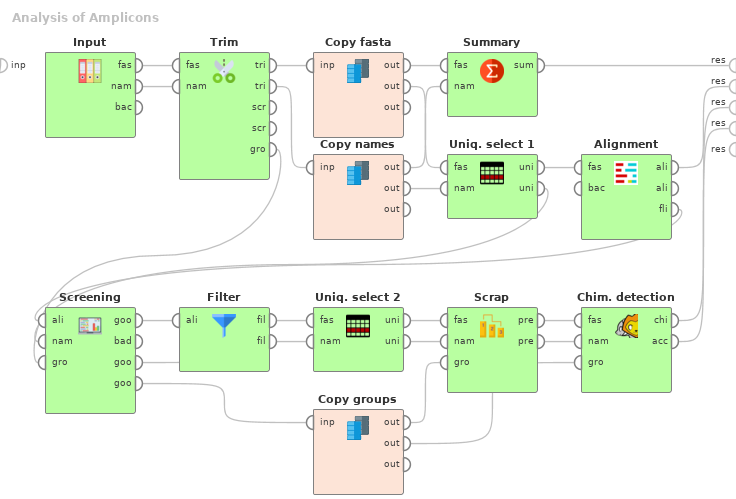
\includegraphics[width=1\linewidth]{Dataflow-color-en.png}
      \end{raggedright}
    \end{column}
    \begin{column}{0.4\textwidth}\footnotesize
      \begin{tabular}{ll}
        Термин & Определение \\
        \hline
        NGS & Секвенирование \\ & нового поколения\\
        Amplicon & Часть ДНК или РНК, \\
               & скопированная  \\
               & много раз \\
        Mothur & Пакет для\\ & исследований в NGS \\
        Rapidminer & Визуальный \\
        studio     & редактор Dataflow-\\
             & диаграмм
      \end{tabular}
      ${}$\\[1em]
      Зеленые блоки -- модули Mothur, другие -- модули Rapidminer studio.
    \end{column}
  \end{columns}
  \vspace{1em}
\end{frame}

\begin{frame}
  \frametitle{Архитектура модулей трансформации}
  \centering
  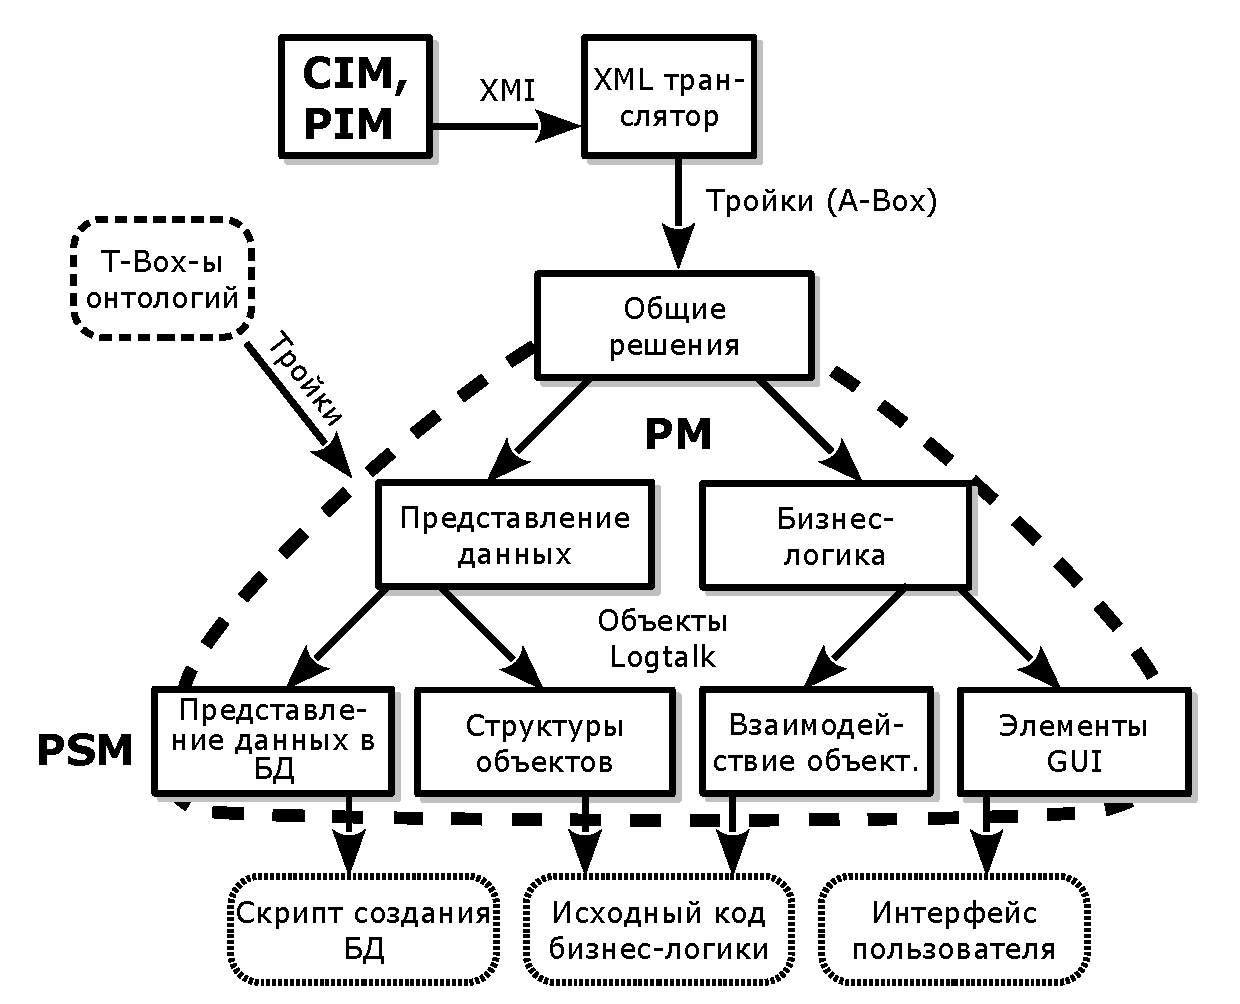
\includegraphics[width=0.9\linewidth]{architect_tree_pres-ru-wo-OCL.pdf}
\end{frame}
\begin{frame}[fragile]
  \frametitle{Сгенерированный модуль Rapidminer studio}
\begin{minted}[fontsize=\tiny]{cpp}
vector<string> AlignCommand::setParameters(){ // PART OF MODULE SOURCE
try {
  CommandParameter ptemplate("reference", "InputTypes", "", "", "none", "none", "none","",false,true,true); parameters.push_back(ptemplate);
  CommandParameter pcandidate("fasta", "InputTypes", "", "", "none", "none", "none","fasta-alignreport-accnos",false,true,true); parameters.push_back(pcandidate);
  CommandParameter psearch("search", "Multiple", "kmer-blast-suffix", "kmer", "", "", "","",false,false,true); parameters.push_back(psearch);
  CommandParameter pksize("ksize", "Number", "", "8", "", "", "","",false,false); parameters.push_back(pksize);
  CommandParameter pmatch("match", "Number", "", "1.0", "", "", "","",false,false); parameters.push_back(pmatch);
// . . . . . . .
\end{minted}
\begin{minted}[fontsize=\tiny]{java}
package com.rapidminer.ngs.operator; // GENERATED JAVA MODULE
// imports

class MothurChimeraCcodeOperator extends MothurGeneratedOperator {
  private InputPort fastaInPort = getInputPorts().createPort("fasta");
  private InputPort referenceInPort = getInputPorts().createPort("reference");
  private OutputPort chimeraOutPort = getOutputPorts().createPort("chimera");
  private OutputPort mapinfoOutPort = getOutputPorts().createPort("mapinfo");
  private OutputPort accnosOutPort = getOutputPorts().createPort("accnos");

  public MothurChimeraCcodeOperator (OperatorDescription description) {
    super(description);
  }
  @Override
  public void doWork() throws OperatorException {
    super();
    // . . . . . .
  }
  @Override
  public List<ParameterType> getParameterTypes() {
    super();
        // . . . . . .
  }
  @Override
  public String getOutputPattern(String type) {
    if (type=="chimera") return "[filename],[tag],ccode.chimeras-[filename],ccode.chimeras";
    if (type=="mapinfo") return "[filename],mapinfo";
    if (type=="accnos") return "[filename],[tag],ccode.accnos-[filename],ccode.accnos";
    return super.getOutputPattern(type);
  }
}
\end{minted}
\end{frame}
\begin{frame}[fragile]
  \frametitle{Представление структуры модулей Mothur в виде графа знаний}
\begin{multicols}{2}
\begin{minted}[fontsize=\tiny]{turtle}
@prefix xml: <http://www.w3.org/XML/1998/namespace> .
@prefix xsd: <http://www.w3.org/2001/XMLSchema#> .
ngsp:spec a ngsp:Specification ;
    ngsp:module mothur:NoCommand,
        mothur:align-check,
        mothur:align-seqs,
# . . . . .
mothur:align-check a ngsp:Module ;
    ngsp:outputPattern [ a cnt:Chars ;
            ngsp:parameterName "type" ;
            ngsp:pattern [ ngsp:patternString
                    "[filename],align.check" ;
                    dc:identifier "aligncheck" ] ;
            cnt:chars # . . . .
# . . . . .
mothur:align-check-idir-parameter a ngsp:Parameter ;
    ngsp:important false ;
    ngsp:multipleSelectionAllowed false ;
    ngsp:optionsDefault "" ;
    ngsp:required false ;
    ngsp:type mothur:String ;
    dc:title "inputdir" .

mothur:align-check-map-parameter a ngsp:Parameter ;
    ngsp:important true ;
    ngsp:multipleSelectionAllowed false ;
    ngsp:optionsDefault "" ;
    ngsp:required true ;
    ngsp:type mothur:InputTypes ;
    dc:title "map" .

mothur:align-check-name-parameter a ngsp:Parameter ;
    ngsp:chooseOnlyOneGroup "namecount" ;
    ngsp:important false ;
    ngsp:multipleSelectionAllowed false ;
# . . . . .
\end{minted}
% \begin{minted}[fontsize=\tiny]{logtalk}
% :- object(queryparam(_RDF_,_Parameter_),
%           extends(ngsquerybase)).

%   :- public(type/1).
%   type(Type) :-
%       ::attr(type, Type).
%   :- public(name/1).
%   name(Name) :- ::attr(dc:title, literal(Name)).
%   :- public(options/1).
%   options(Value):- ::attr(options, Value).
%   :- public(options_default/1).
%   options_default(Value):-
%     ::attr(optionsDefault, Value).
%   % . . . . . . . .
%   :- public(multiple_selection_allowed/0).
%   multiple_selection_allowed:-
%     ::bool_attr(multipleSelectionAllowed).
%   :- public(required/0).
%   required:-
%     ::bool_attr(required).
%   :- public(important/0).
%   important:-
%     ::bool_attr(important).
%   :- protected(attr/2).
%   attr(NS:Name, Value):-
%     ::second(Parameter),
%     rdf_db::rdf_global_object(Value, V),
%     _RDF_::rdf(Parameter, NS:Name, V).
%   attr(Name, Value):-
%     \+ Name=_:_,!,
%     ::second(Parameter),
%     rdf_db::rdf_global_id(Value, V),
%     _RDF_::rdf(Parameter, ngsp:Name, V).
%   % . . . . .
% :- end_object.

% \end{minted}
\end{multicols}
\end{frame}
\begin{frame}
  \frametitle{Инфраструктура сервисов}
  \centering
  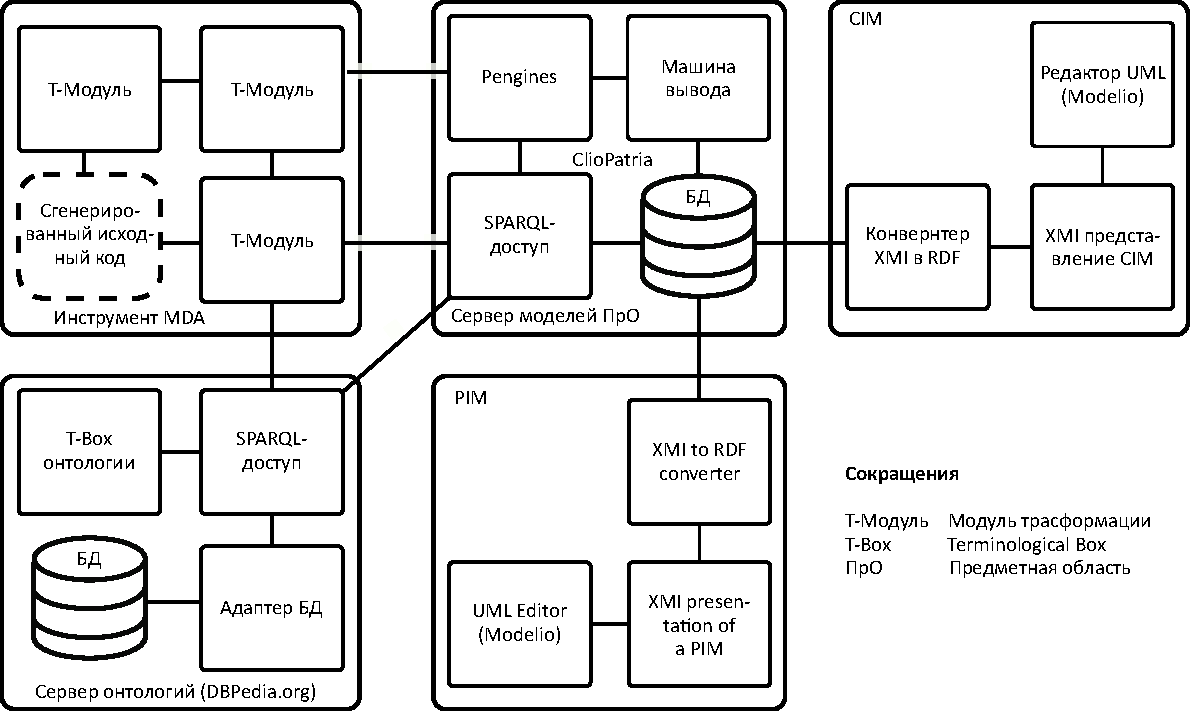
\includegraphics[width=1\linewidth]{architecture-mda-lod-ext-ru.pdf}
\end{frame}
\begin{frame}
  \frametitle{Язык Logtalk}
  Язык Logtalk выбран в качестве языка представления трансформаций по следующим причинам:
  \begin{itemize}
  \item наследует все свойства сред программирования \textbf{ISO-Prolog};
  \item реализован в виде \textbf{макропакета}; накладные расходы в случае использования только статических объектов -- 1.5\%;
  \item гибкий подход к представлению трансформаций: синтаксически одинаково задаются как трансформации, так и ограничения;
  \item параметрические объекты (\texttt{circle(0,0,10)::square(S)}).
  \item реализация ОО-представления базы знаний (правил): структуризация, инкапсуляция, замена части и т.п.;
  \item представление объектов-трансформаций как композиций при помощи категорий;
  \item механизмы фильтрации при передаче сообщений;
  \item представлены реализации для разных ISO-Prolog-систем.
  \end{itemize}
  % The <<regular>> language allow us to use its libraries not directly related to MDA transformations.
\end{frame}
% \begin{frame}
%   \frametitle{Model Driven Architecture и Linked Open Data}
%   \begin{center}
%     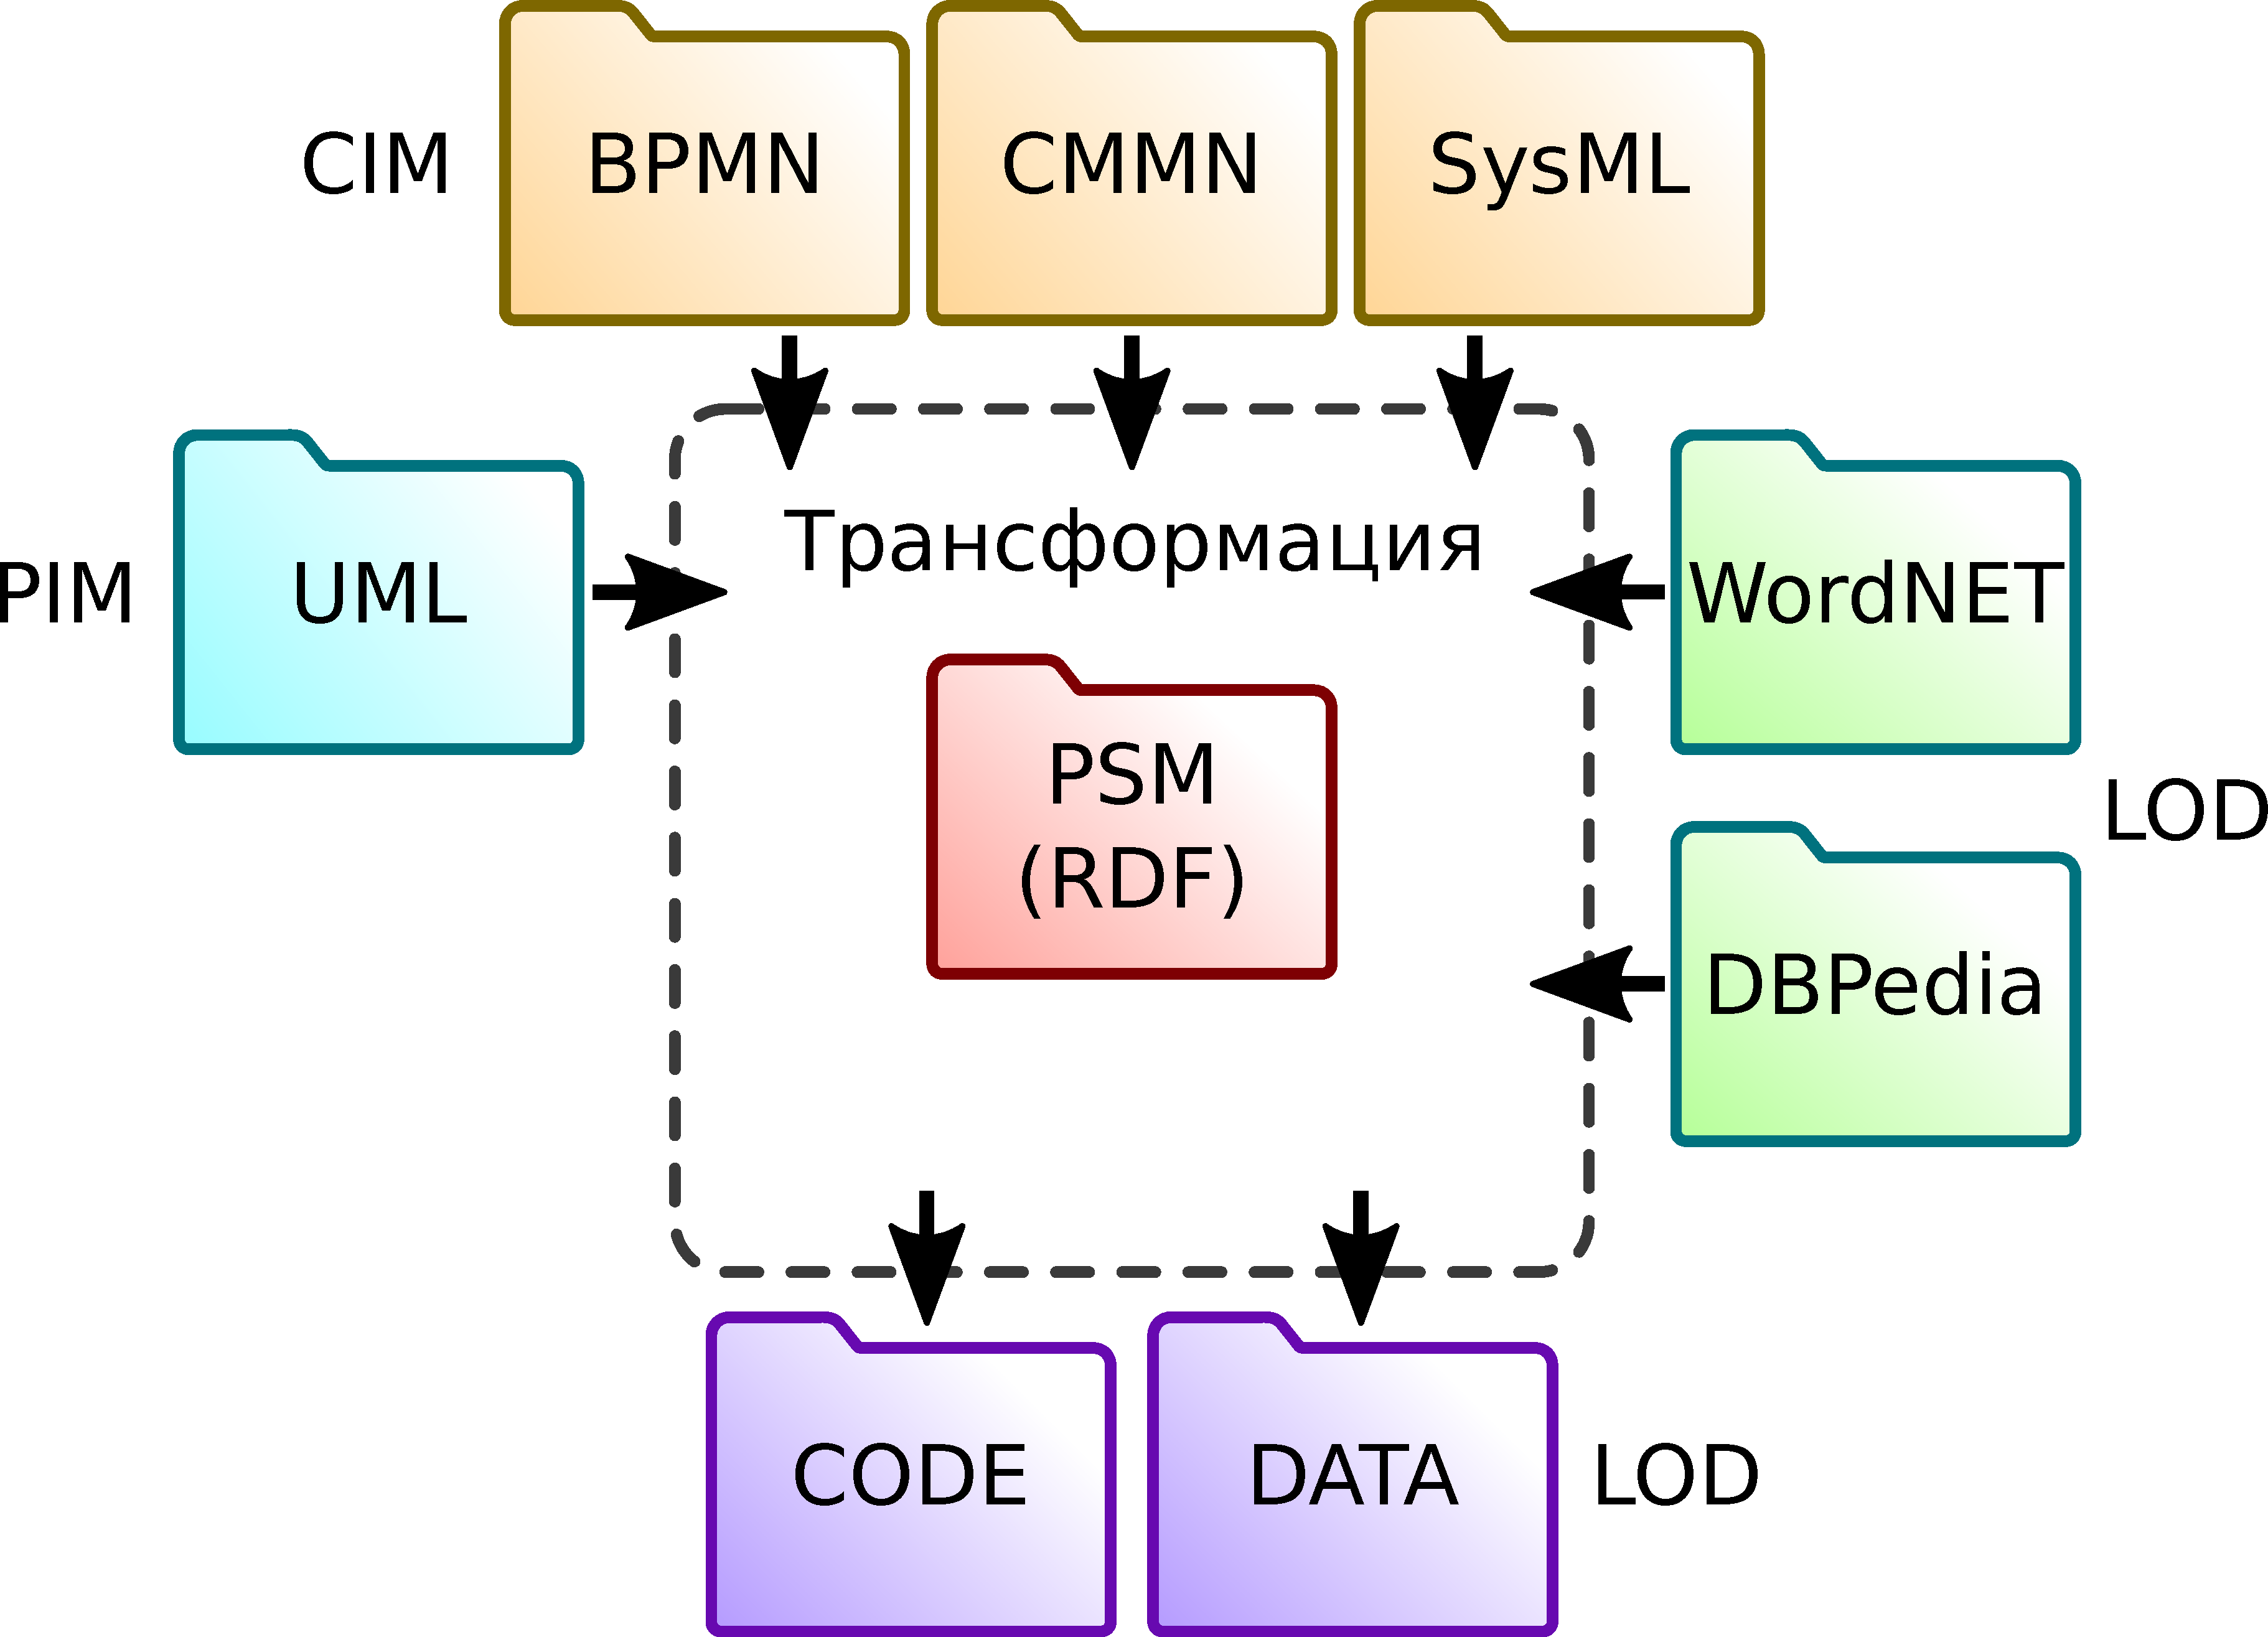
\includegraphics[width=0.9\linewidth]{mda-overview-ru.pdf}
%   \end{center}
% \end{frame}
\begin{frame}[fragile]
  \frametitle{Применение SW для представления моделей}
  \begin{itemize}
  \item Использование накопленного опыта и стандартов формализации предметных областей;
  \item Представление T-Box и A-Box при помощи множества троек (графа) \texttt{<субъект, отношение, объект>};
  \item Элементы стандартных онтологий формально описаны (\verb|rdfs:domain|, \verb|rdfs:range|);
  \item Поддерживаются большинством программных систем (библиотеки, системы логического вывода, SPARQL);
  \item Предлагает способ глобальной идентификации объектов в различных независимых системах;
  \item SWI-Prolog включает библиотеку, позволяющую осуществлять запросы к графу, интерпретацию семантики некоторых отношений (\verb|rdfs:label|, \verb|dc:title|), инкапсуляцию BNode в многоаргументные предикаты; сервер онтологий ClioPatria;
  \item Предоставляется простой способ разделения уровней доступа к информации: (\verb|rdfs:seeAlso|);
  \item Разметка RDF/LOD позволяет интегрировать гетерогенные системы.
  \end{itemize}
\end{frame}
\begin{frame}[fragile]
  \frametitle{Сценарий синтеза класса по сценарию}

%\begin{multicols}{2}
  \begin{columns}
    \begin{column}{0.6\textwidth}
\begin{minted}[fontsize=\tiny]{logtalk}
:- object(script(_Package_,_LocalProf_,_CodeProf_)). % Трансформационный профиль
  :- public([tr/4,tr/3]).                            % Публичный интерес сценария
  % . . . . . . . . . .
  tr(class, Class, ClassID):-   % Синтез класса
    % Запрос к структурам пакета
    query(_Package_)::class(Name, ClassID),
    create_object(Class, . . . . .% Создание объекта <<Класс>>
    create_object(Attributes,. . .% Создание атрибута
    create_object(Methods, . . . .% ... метода
    Class::name(Name),            % Поименование класса
    % Порождение атрибутов класса,
    % Представление их в виде локальной базы данных.
    % ... то же с методами ...
    Class::attributes(Attributes),  % Ассоциация атрибутов с классом
    Class::methods(Methods).        % ... и методов тоже..

    % Трансформация атрибутов
  tr(attribute, Attribute, ClassID, AttributeID):-
    query(_Package_)::attribute(Name,ClassID,AttrID),
    create_object(Attribute,  % . . . . .
    Attribute::name(Name).    % Поименование атрибута

    % Трансформация метода
  tr(method, Method, ClassID, MethodID):-
    query(_Package_)::method(Name,ClassID,MethodID),
    create_object(Method,     % . . . . .
    Method::name(Name).       % Поименование метода
  . . . . . . . . . . . . . . .
  tr :-                       % Запуск АКИД
    forall( tr(class, Class, ClassID),
         ( forall(tr(attribute, A, ClassID, AID), true),
           forall(tr(method, M, ClassID, MID), true)).
:- end_object.
\end{minted}
    \end{column}
    \begin{column}{0.4\linewidth}
      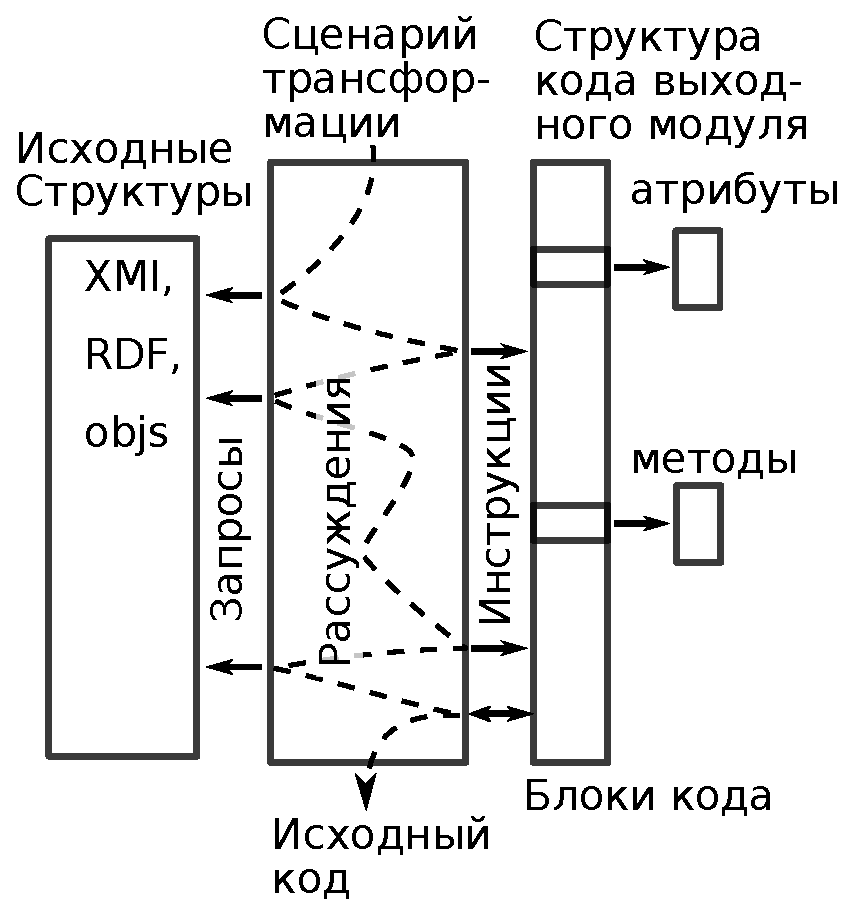
\includegraphics[width=1\linewidth]{scenario-ru-wo-mothur.pdf}
    \end{column}
  \end{columns}
  % \end{multicols}
\end{frame}

\begin{frame}[fragile]
  \frametitle{Реализация объекта-фасада \texttt{query}}
\begin{minted}[fontsize=\footnotesize{}]{logtalk}
:- object(query(_XMI_)).

  :- public([class/2, attribute/3, method/3]).
  class(Name, ID):-                            % Распознавание
    _XMI_::rdf(ID,rdf:type,uml:'Class'),       % класса
    _XMI_::rdf(ID,rdfs:label, literal(Name)).

  attribute(Name, ClassID, ID):-               % ...атрибута...
    _XMI_::rdf(ClassID, xmi:ownedAttribute, ID),
    _XMI_::rdf(ID, rdfs:label, literal(Name)).

  method(Name, ClassID, ID):-                  % ...метода...
    _XMI_::rdf(ClassID, xmi:ownedOperation, ID),
    _XMI_::rdf(ID, rdfs:label, literal(Name)).
  % . . . . . . . . . . .
:- end_object.
\end{minted}
\end{frame}

\begin{frame}[fragile]
\frametitle{Блок кода (интерпретация объекта)}
 Идея реализации взята из \texttt{llvmlite}${}^*$)
  \begin{columns}
    \begin{column}{0.6\textwidth}
      \flushleft
\begin{minted}[fontsize=\footnotesize{}]{logtalk}
:- object(code_block, specializes(root)).
  % Публичный интерфейс объекта
  :- public([append/1, prepend/1, clear/0,
    render/1, render_to/1, remove/1,
    item/1, items/1]).
  % Элементы блока
  :- dynamic([item_/1]).
  :- private([item_/1]).
  % Специализации методов при наследовании
  :- protected([renderitem/2, render_to/2]).
  % Позволить объекту сгенерировать
  % свое представление самостоятельно
  renderitem(Object, String):-
    current_object(Object), !,
    Object::render(String).
  % Преобразовать литерал в строку
  renderitem(literal(Item), String):-!,
    atom_string(Item, String).
  % Отобразить как есть (для отладки).
  renderitem(Item, String):-
    root::iswritef(String, '%q', [Item]).
:- end_object.
\end{minted}
    \end{column}
    \begin{column}{0.4\textwidth}
      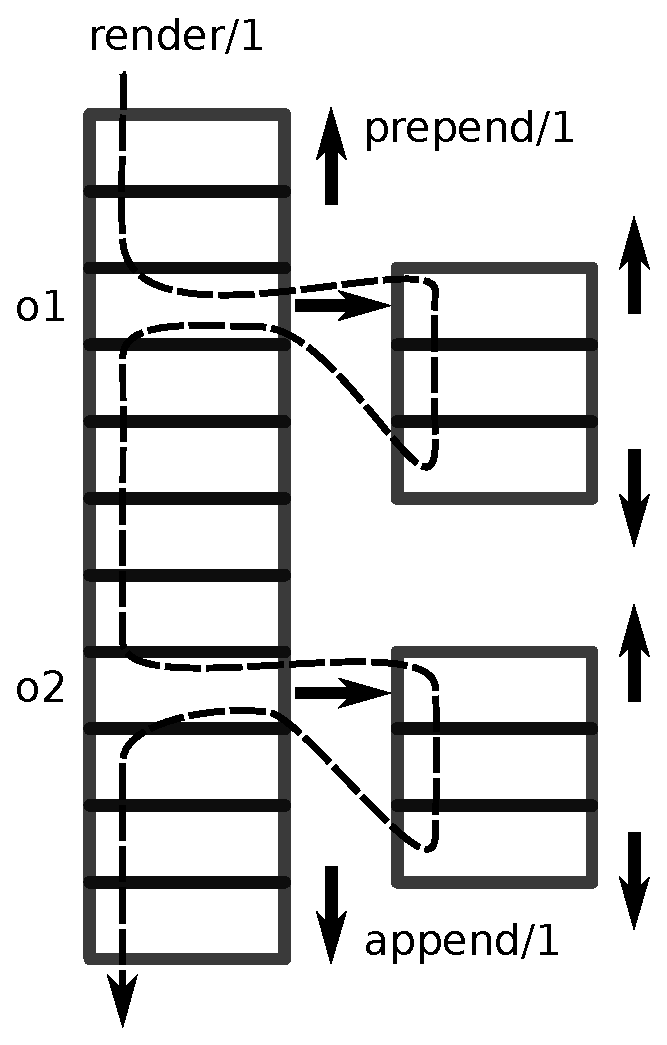
\includegraphics[width=1\linewidth]{code_block.pdf}
  ${}^*$) \url{https://github.com/numba/llvmlite}
    \end{column}
  \end{columns}
\end{frame}

\begin{frame}[fragile]
  \frametitle{Модель класса Python (пример)}
%\begin{multicols}{2}
  \begin{columns}
    \begin{column}{0.6\textwidth}
      \flushleft
\begin{minted}[fontsize=\scriptsize]{logtalk}
:- object(class, specializes(code_block),
   imports([named])). % Категория поименованных сущностей
  :- public([classlist/1, methods/1, attributes/1]).
  % . . . . . . . . . . . . . .
  renderitem(Item, Result):-    % Стандартное
    ^^renderitem(Item, Result). % преобразование
  render(Result):-       % Генератор кода, реализо-
    ^^render(Name),      % ванный в категории
    ( ::item(classlist(List)) ->
     % . . . . . . . . . . .
        [Name]) ),
    ( ::item(attributes(Attributes))->
     % . . . . . . . . . . .
        [DefAttrList]),
      Attributes::items(InstanceAttrs),
      findall(S, ( % Инициализация атрибутов
         % . . . . . . . . .
         ), AttrAssigns),
        root::unindent,
        AttrList=[ConstructorDef|AttrAssigns];
         % . . . . . . . . .
        AttrList=[ConstructorDef, Pass] ),
    ( ::item(methods(Methods))-> % Если есть ...
      Methods::render(MethodList);
      MethodList=[] ),
    lists::append(AttrList,MethodList,StringList),
    root::unindent, Result=[Signature|StringList].
:- end_object.
\end{minted}
    \end{column}
    \begin{column}{0.4\linewidth}
      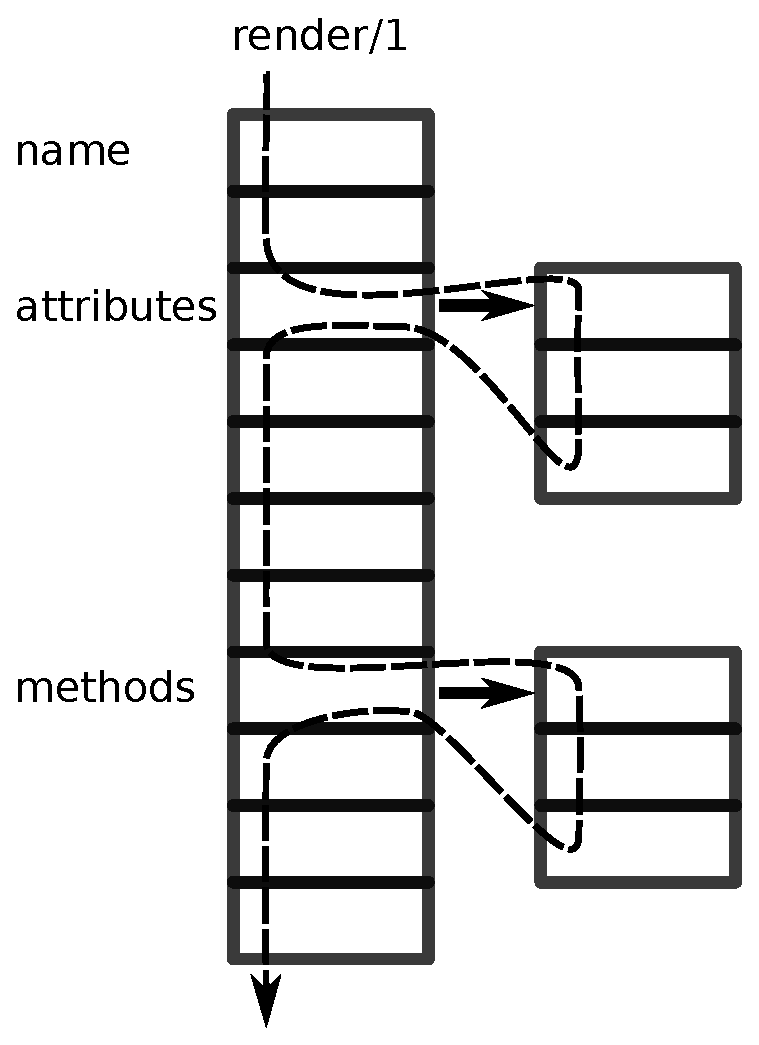
\includegraphics[width=1\linewidth]{code_block_class.pdf}
    \end{column}
  \end{columns}
  % \end{multicols}
\end{frame}

\begin{frame}[fragile]
  \frametitle{Категории Logtalk}
  Категория поименованных сущностей
\begin{minted}[fontsize=\scriptsize]{logtalk}
:- category(named).
  :- public([name/1, render/1]).
  :- protected([renderitem/2]).
  name(Name):- ::prepend(name(Name)).
  renderitem(name(Name), String):-!, atom_string(Name, String).
  render(String):-  % Порождение кода
    ::item(name(Name)), ::renderitem(name(Name), String).
:-end_category.
\end{minted}
Категория поименованных типизированных сущностей
\begin{minted}[fontsize=\scriptsize]{logtalk}
:- category(namedtyped, extends(named)).
  :- public([type/1,render/2, separator_option/2,list_separator/1]).
  :- protected([renderitem/2]).
  type(Type):- ::append(type(Type)).
  renderitem(Item, String):- ^^renderitem(Item, String),!.
  renderitem(type(Type),String):-!, ::list_separator(Separator),
    writef::swritef(String, '%w%w', [Separator, Type]).
  render(Middle, String):- ^^render(SName),
    ( ::item(type(Type)) ->
      ::renderitem(type(Type), SType),
      string_concat(SName, Middle, _1),
      string_concat(_1, SType, String) ;
      SName = String ).
  render(String):-  ::render("", String).
  list_separator(Separator):-
      ::separator_option(Name, Default),!, % Глобальные настройки
      root::option(Name, Separator, Default).
:- end_category.
\end{minted}
\end{frame}

\begin{frame}[fragile]
  \frametitle{Доступ к внешним графам знаний, LOD}

  \begin{columns}
\begin{column}{0.5\textwidth}
\begin{minted}[fontsize=\scriptsize]{logtalk}
:- category(sparql).
  :- public(query/2).
  query(Pattern,Parameters,Row):-
    prepare(Pattern,Parameters,Query),
    server(Host,Port,Path),
    sparql_query(Query, Row,
      [host(Host),port(Port),path(Path)]).
   :- protected(server/3).  % реализовать
                           % при наследовании.
  :- protected(prepare/3). % подготовка запроса
  % . . . . . . . . . .    % в виде строки.
  :- end_category.

  :- object(dbpedia, extends(sparql)).
  :- protected(server/3).
  server('dbpedia.org',80,'/sparql').
  :- public(entity_name/2).
  entity_name(Entity,Language,Name):-
    query('select ?name where { '
      ' %w rdfs:label ?name. '
      'FILTER langMatches( lang(?label),'
      ' "%w" )}', [Entity, Language],
      row(Name)).
:- end_object.

% ?- dbpedia::entity_name(dbr:'Passport', 'ru', Name).
\end{minted}
\end{column}
\begin{column}{0.5\textwidth}
  \flushright
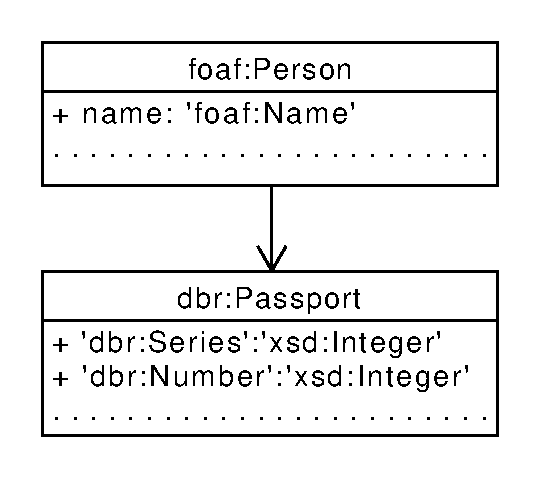
\includegraphics[width=0.8\linewidth]{simple-diag.pdf}
\end{column}
\end{columns}
\end{frame}


\begin{frame}
  \frametitle{Обсуждение}
  Интересные замечания по поводу использования Logtalk:
  \begin{itemize}
  \item Logtalk и RDF гибки и достаточно универсальны для удобной реализации задач АКИД, выразимые в терминах анализа свойств и преобразования элементов
  \item Наиболее полезным средством Prolog и Logtalk -- предикатная и объектная инкапсуляция: сложные рассуждения можно скрыть за интерфейсами
  \item Необходимо дальнейшее изучение свойств языка (2009).
  \end{itemize}

  \begin{itemize}
  \item {\color{mymauve} В настоящий момент ведется НИРОКР в области распознавания структуры текста в PDF"=документе, в частности в учебных программ вузов и их RDFa"=разметки.}
  \item {\color{mymauve} Для размеченного инструмента разрабатывается веб-сервис редактирования компонент текста с учетом их семантики (текст, перечисление, иерархический список, ссылка на литературу и т.п.)}
  \end{itemize}
\end{frame}

\begin{frame}
  \frametitle{Заключение}
  Результаты, полученные к настоящему времени:
  \begin{itemize}
  \item Разработаны методики представления алгоритмов распознавания текстовых структур.
  \item Разработана методика представления сценариев распознавания и трансформации в виде иерархии логических объектов.
  \item Накоплен некоторый опыт реализации конкретных задач в области порождения кода информационных систем и анализа слабоструктурированных документов.
  \item Существенных технических проблем пока не выявлено.
  \end{itemize}
  Дальнейшее развитие проекта:
  \begin{itemize}
  % \item Создание удобных для программиста инструментов семантической LOD-разметки форм и документов.
  \item Разработка методик программирования с преимущественным использованием статических объектов.
  \item Реализация библиотек и для конкретных классов задач.
  \end{itemize}
  Исходные коды находятся на Github в разделах:
  \begin{itemize}
  \item \url{https://github.com/isu-enterprise},
  \item \url{https://github.com/eugeneai}.
  \end{itemize}
\end{frame}

\begin{frame}
  \begin{center}
  \Large Спасибо за уделенное внимание!
\end{center}
\end{frame}

\begin{frame}
  \frametitle{Приложение: Представление NGS в виде диаграммы DataFlow}
  \begin{columns}
    \begin{column}{0.6\textwidth}
      \begin{raggedright}
        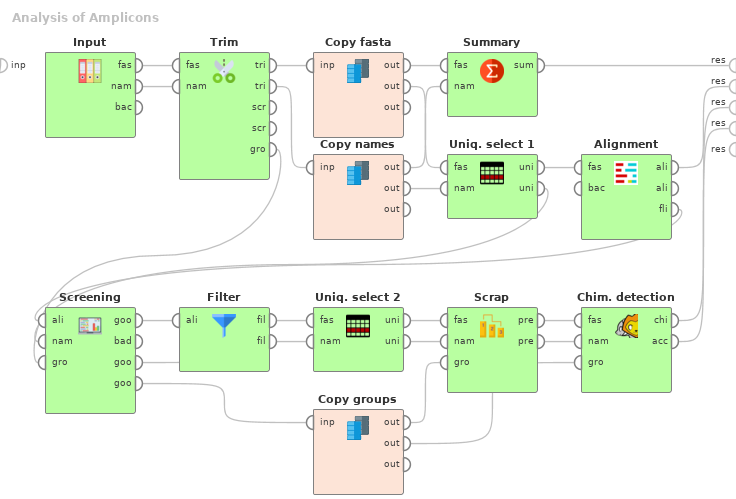
\includegraphics[width=1\linewidth]{Dataflow-color-en.png}
      \end{raggedright}
    \end{column}
    \begin{column}{0.4\textwidth}\footnotesize
      \begin{tabular}{ll}
        Термин & Определение \\
        \hline
        NGS & Секвенирование \\ & нового поколения\\
        Amplicon & Часть ДНК или РНК, \\
               & скопированная  \\
               & много раз \\
        Mothur & Пакет для\\ & исследований в NGS \\
        Rapidminer & Визуальный \\
        studio     & редактор Dataflow-\\
             & диаграмм
      \end{tabular}
      ${}$\\[1em]
      Зеленые блоки -- модули Mothur, другие -- модули Rapidminer studio.
    \end{column}
  \end{columns}
  \vspace{1em}
  Использование MDA позволяет актуализировать структуру ПП Mothur (в н.в. 144 модуля).
\end{frame}


\end{document}

%%% Local Variables:
%%% mode: latex
%%% TeX-master: t
%%% End:
